\section{System}
Die Benutzung von MArC ist in der dem Programm mitgelieferten ReadMe-Datei beschrieben. Darin wird erklärt, welche Hard- und Software komponenten erforderlich sind, wie das System gestartet und kalibriert wird. Des weiteren enthält die ReadMe eine Übersicht über die enthaltenen Quellcode-Dateien.
\subsection{Starten des Systems}
Nachdem sichergestellt wurde, dass alle in der ReadMe-Datei beschriebenen Voraussetzungen bestehen, kann das System gestartet werden, indem zunächst die Tracking-Anwendung (auf dem einen Computer) und anschließend die aus Unity heraus erstellte Anwendung (auf dem anderen Computer) gestartet wird. Auf letzterem Computer beginnt darauffolgend die Menüführung, welche in \ref{sec:menu} beschrieben ist. 
\subsection{Menüführung}\label{sec:menu}
Die Menüführung dient dazu, den Benutzer durch alle notwendigen Schritte zu leiten, die vor dem Starten der eigentlichen Simulation erforderlich sind.

Die folgenden Menüs sind Bestandteil der Menüführung:\todo[inline]{Screenshots der Menüs einfügen?}
\begin{description}
	\item[\texttt{CalibDone}:] Wird aufgerufen, wenn die Kalibrierung des Arbeitsbereichs abgeschlossen ist. Es informiert den Benutzer, dass die Kalibrierung erfolgreich war und der Vorgang fortgesetzt werden kann.
	\item[\texttt{CalibrateOrNot}:] Erscheint nach dem Verlassen des \texttt{Welcome}-Menüs und erlaubt dem Benutzer eine Kalibrierung durchzuführen oder eine bereits durchgeführte Kalibrierung zu laden.
	\item[\texttt{ControllerNotFound}:] Warnt den Benutzer nach dem Starten der Kalibrierung, dass der HTC Vive Controller, welcher für die Kalibrierung benötigt wird, nicht eingeschaltet ist. Während das Menü angezeigt wird, kann der Benutzer den Controller einschalten und anschließend auf \texttt{Continue} klicken.
	\item[\texttt{SelectCalibrationTarget}:] Erlaubt die Auswahl der Art der Kalibrierung. Es kann hier entweder nur der Arbeitsbereich oder sowohl der Arbeitsbereich, als auch die Kamera kalibriert werden. Die Kalibrierung ist näher in \ref{sec:calib} beschrieben.
	\item[\texttt{SetScale}:] Stellt das letzte Menü vor dem Starten der Simulation dar. In diesem kann der Benutzer den Maßstab der Gebäudesimulation einstellen und anschließend die Simulation starten.
	\item[\texttt{SocketNotReady}:] Warnt den Benutzer nach dem Verlassen des \texttt{Welcome}-Menüs, dass die Netzwerkverbindung zum Computer, auf dem die Tracking-Anwendung ausgeführt wird, nicht bereit ist. Nach Bestätigung dieses Hinweises durch einen Klick auf \texttt{Continue}, kehrt der Benutzer zum \texttt{Welcome}-Menü zurück. Anschließend kann der Vorgang fortgesetzt werden, wenn die Netzwerkverbindung hergestellt wurde. Andernfalls erscheint wieder \texttt{SocketNotReady}.
	\item[\texttt{Welcome}:] Erscheint als erstes Menü. Hier erhält der Nutzer eine kurze Information darüber, wie die Anwendung heißt und wozu sie dient.
	\item[\texttt{doPlaneCalibInVS}:] Dient dem Benutzer als Anleitung für die Durchführung der Arbeitsbereich-Kalibrierung. Diese wird in \ref{sec:planeCalib} genauer beschrieben.
	\item[\texttt{doPoseCalibInVS}:] Dient dem Benutzer als Anleitung für die Durchführung der Kamera-Kalibrierung. Diese wird in \ref{sec:camCalib} genauer beschrieben.
\end{description}

\begin{figure}[htbp]
	\centering
	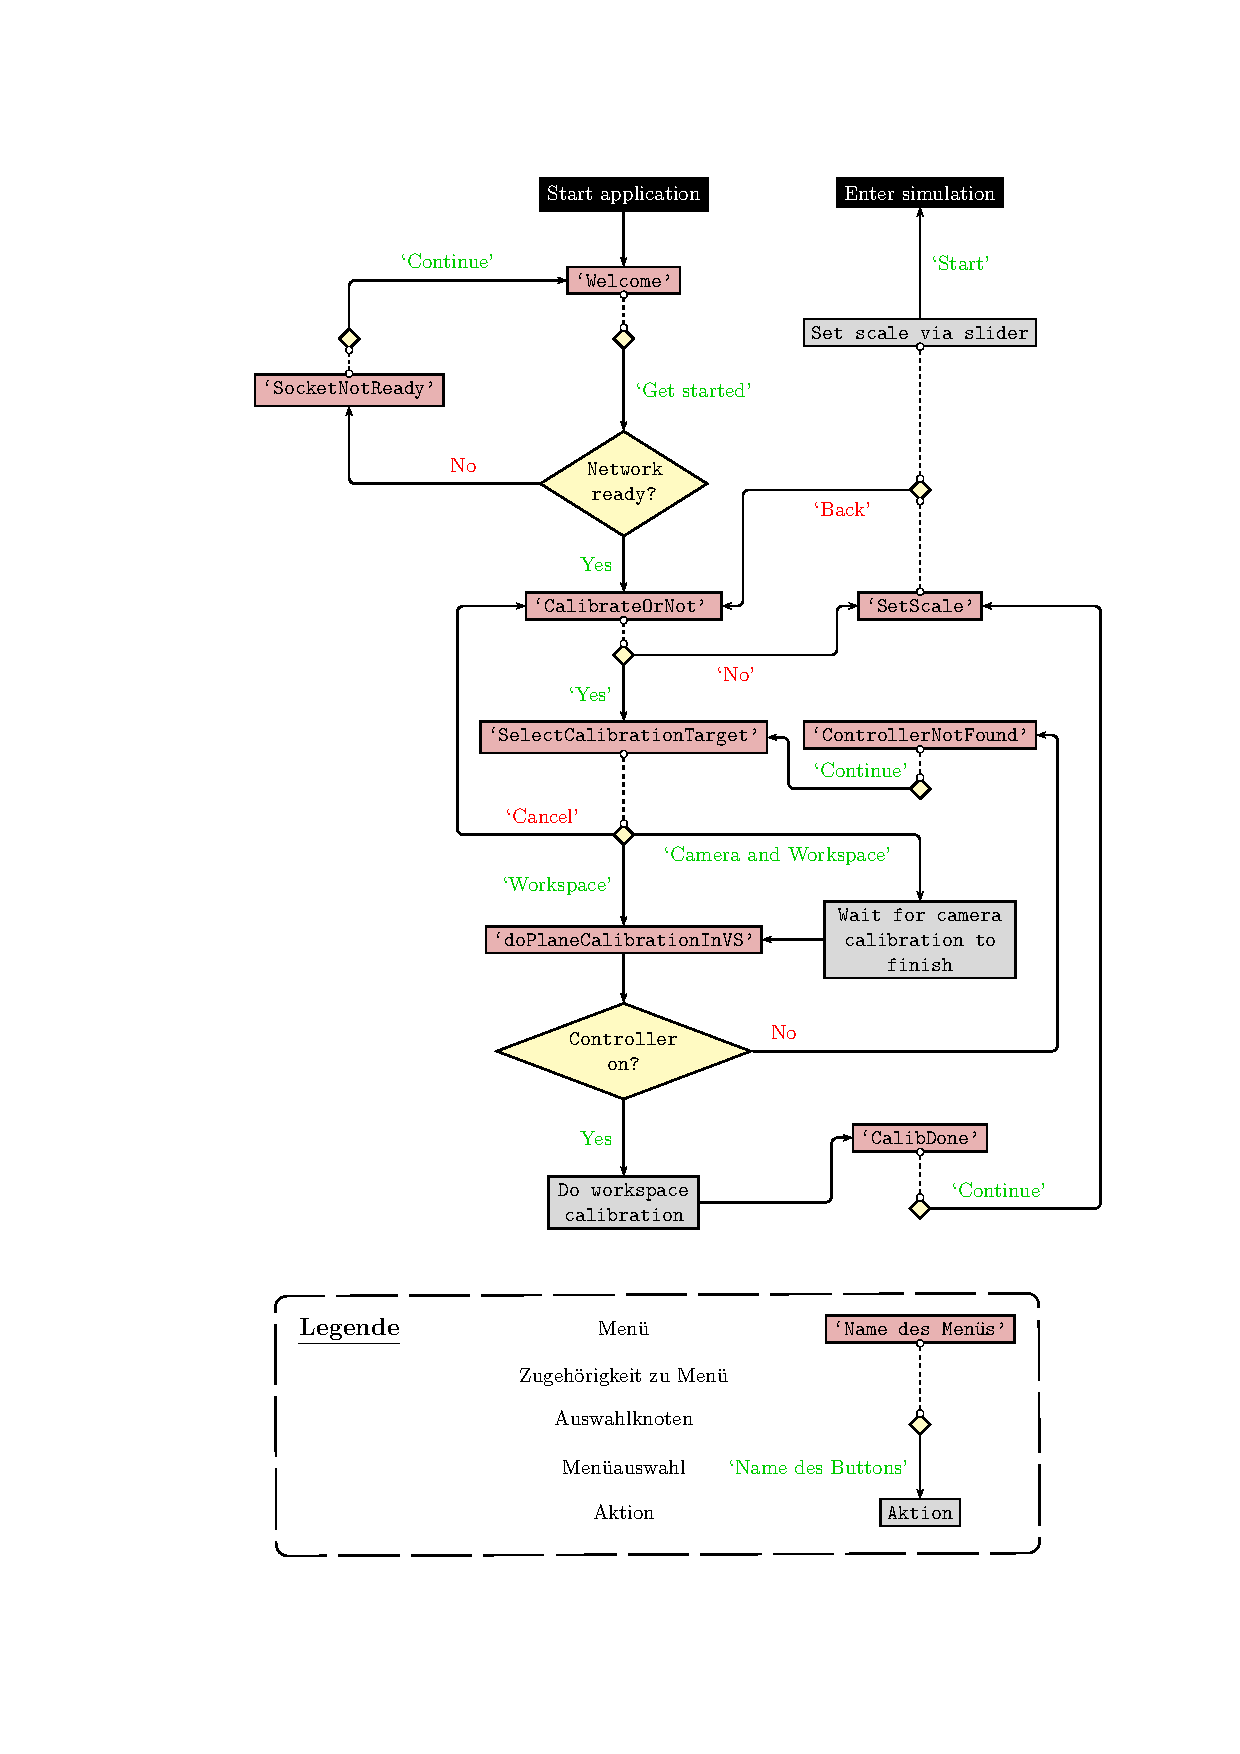
\includegraphics[scale=.9, trim=5cm 2.5cm 3.5cm 2.5cm]{kapitel/system/MP_Menu_Flowchart.pdf}
	\caption{Flussdiagramm der Menüführung.}
\end{figure}
\subsection{Kalibrierung}\label{sec:calib}
Um das Ziel von MArC zu erreichen, an den Positionen der Aluminiumwürfel im Arbeitsbereich in der virtuellen Realität von Unity gerenderte Würfel darzustellen, muss das System kalibriert werden. Die Kalibrierung hat zum Ziel, eine Koordinatentransformation zu finden, die Positionen im Kamera-Koordinatensystem in das Unity-Koordinatensystem transformiert.

Zu diesem Zweck muss eine zweistufige Kalibrierung durchgeführt werden. Zunächst sorgt die Kamerakalibrierung dafür, dass Bildkoordinaten auf dem Sensor der Kamera in das 3D-Kamera-Koordinatensystem transformiert werden. Dafür wird sich einiger OpenCV-Funktionen in Verbindung mit AruCo-Markern bedient. Dieser Vorgang wird nachfolgend in~\ref{sec:camCalib} genauer beschrieben.\\
Der nächste Schritt, die Kalibrierung des Arbeitsbereichs, bestimmt über Punkt-Korrespondenzen -- also in zwei verschiedenen Koordinatensystemen bekannte Punkte -- eine affine 3D-Transformation, welche die Abbildung vom Kamera-Koordinatensystem auf das Unity-Koordinatensystem ermöglicht. Dieser Kalibrierungsschritt wird nachfolgend in~\ref{sec:planeCalib} näher beschrieben.\\
Trotz einer sorgfältigen Umsetzung der in den nächsten beiden Kapiteln beschriebenen Kalibrierungsschritte, ist es nicht gelungen, den Aluminiumwürfel und den gerenderten Würfel vollständig zur Deckung zu bringen. Der entstandene Fehler sowie mögliche systembedingte Fehlerquellen werden in~\ref{sec:calibError} und in~\ref{sec:calibErrorSources} beschrieben. 

\subsubsection{Kamerakalibrierung}\label{sec:camCalib}
wie in \cite{Meisel:77890}.


\subsubsection{Kalibrierung des Arbeitsbereichs}\label{sec:planeCalib}
\subsubsection{Kalibrierungfehler} \label{sec:calibError}
\subsubsection{Mögliche Fehlerquellen} \label{sec:calibErrorSources}


